% Options for packages loaded elsewhere
\PassOptionsToPackage{unicode}{hyperref}
\PassOptionsToPackage{hyphens}{url}
%
\documentclass[
  ignorenonframetext,
  aspectratio=169]{beamer}
\title{Principles of field plot experiments}
\author{Deependra Dhakal}
\date{}
\institute{Assistant Professor \and Agriculture and Forestry
University \and \url{https://rookie.rbind.io}}

\usepackage{pgfpages}
\setbeamertemplate{caption}[numbered]
\setbeamertemplate{caption label separator}{: }
\setbeamercolor{caption name}{fg=normal text.fg}
\beamertemplatenavigationsymbolsempty
% Prevent slide breaks in the middle of a paragraph
\widowpenalties 1 10000
\raggedbottom
\setbeamertemplate{part page}{
  \centering
  \begin{beamercolorbox}[sep=16pt,center]{part title}
    \usebeamerfont{part title}\insertpart\par
  \end{beamercolorbox}
}
\setbeamertemplate{section page}{
  \centering
  \begin{beamercolorbox}[sep=12pt,center]{part title}
    \usebeamerfont{section title}\insertsection\par
  \end{beamercolorbox}
}
\setbeamertemplate{subsection page}{
  \centering
  \begin{beamercolorbox}[sep=8pt,center]{part title}
    \usebeamerfont{subsection title}\insertsubsection\par
  \end{beamercolorbox}
}
\AtBeginPart{
  \frame{\partpage}
}
\AtBeginSection{
  \ifbibliography
  \else
    \frame{\sectionpage}
  \fi
}
\AtBeginSubsection{
  \frame{\subsectionpage}
}
\usepackage{amsmath,amssymb}
\usepackage{lmodern}
\usepackage{iftex}
\ifPDFTeX
  \usepackage[T1]{fontenc}
  \usepackage[utf8]{inputenc}
  \usepackage{textcomp} % provide euro and other symbols
\else % if luatex or xetex
  \usepackage{unicode-math}
  \defaultfontfeatures{Scale=MatchLowercase}
  \defaultfontfeatures[\rmfamily]{Ligatures=TeX,Scale=1}
\fi
\usetheme[]{Frankfurt}
\usecolortheme{beaver}
% Use upquote if available, for straight quotes in verbatim environments
\IfFileExists{upquote.sty}{\usepackage{upquote}}{}
\IfFileExists{microtype.sty}{% use microtype if available
  \usepackage[]{microtype}
  \UseMicrotypeSet[protrusion]{basicmath} % disable protrusion for tt fonts
}{}
\makeatletter
\@ifundefined{KOMAClassName}{% if non-KOMA class
  \IfFileExists{parskip.sty}{%
    \usepackage{parskip}
  }{% else
    \setlength{\parindent}{0pt}
    \setlength{\parskip}{6pt plus 2pt minus 1pt}}
}{% if KOMA class
  \KOMAoptions{parskip=half}}
\makeatother
\usepackage{xcolor}
\IfFileExists{xurl.sty}{\usepackage{xurl}}{} % add URL line breaks if available
\IfFileExists{bookmark.sty}{\usepackage{bookmark}}{\usepackage{hyperref}}
\hypersetup{
  pdftitle={Principles of field plot experiments},
  pdfauthor={Deependra Dhakal},
  hidelinks,
  pdfcreator={LaTeX via pandoc}}
\urlstyle{same} % disable monospaced font for URLs
\newif\ifbibliography
\setlength{\emergencystretch}{3em} % prevent overfull lines
\providecommand{\tightlist}{%
  \setlength{\itemsep}{0pt}\setlength{\parskip}{0pt}}
\setcounter{secnumdepth}{-\maxdimen} % remove section numbering
\usepackage{setspace}
\usepackage{wasysym}
\usepackage{fontenc}
\usepackage{booktabs,siunitx}
\usepackage{longtable}
\usepackage{array}
\usepackage{multirow}
\usepackage{wrapfig}
\usepackage{float}
\usepackage{colortbl}
\usepackage{pdflscape}
\usepackage{tabu}
\usepackage{threeparttable}
\usepackage{threeparttablex}
\usepackage[normalem]{ulem}
\usepackage{makecell}
\usepackage{xcolor}
\usepackage{tikz} % required for image opacity change
\usepackage[absolute,overlay]{textpos} % for text formatting
\usepackage[skip=0.3\baselineskip]{caption}
% \usepackage{newtxtext,newtxmath}% better than txfonts   

% this font option is amenable for beamer
\setbeamerfont{caption}{size=\tiny}
\singlespacing

\sisetup{per-mode=symbol}

\newcommand\Myperm[2][^n]{\prescript{#1\mkern-2.5mu}{}P_{#2}}
\newcommand\Mycomb[2][^n]{\prescript{#1\mkern-0.5mu}{}C_{#2}}

% \setcounter{totalnumber}{50}
% \setcounter{topnumber}{50}
% \setcounter{bottomnumber}{50}
% \setlist[itemize,1]{leftmargin=2pt,itemindent=2pt}
% \setlist[itemize,2]{leftmargin=6pt,itemindent=2pt}
% \def\labelitemi{$\bullet$}
% \def\labelitemii{$\diamond$}
% \def\labelitemiii{\textbullet}
\setbeamerfont{caption}{size=\tiny}
\setbeamertemplate{footline}[page number]
\AtBeginSection{}
\AtBeginSubsection{}
\setbeamersize{text margin left=5mm,text margin right=5mm}
\newcommand{\bcolumns}{\begin{columns}[T, onlytextwidth]}
\newcommand{\ecolumns}{\end{columns}}
\newcommand{\bdescription}{\begin{description}}
\newcommand{\edescription}{\end{description}}
\ifLuaTeX
  \usepackage{selnolig}  % disable illegal ligatures
\fi

\begin{document}
\frame{\titlepage}

\begin{frame}[allowframebreaks]
  \tableofcontents[hideallsubsections]
\end{frame}
\hypertarget{principles-of-field-plot-experiments}{%
\section{Principles of field plot
experiments}\label{principles-of-field-plot-experiments}}

\begin{frame}{}
\protect\hypertarget{section}{}
\begin{quote}
To call the statistician after the experiment may be no more than asking him to perform a postmortem examination ...\\[1cm]

... he may be able to say what the experiment died of. 

\end{quote}

\hfill \raggedright -- R.A. Fisher, 1938
\end{frame}

\begin{frame}{}
\protect\hypertarget{section-1}{}
\footnotesize

\begin{itemize}[<+->]
\tightlist
\item
  A new drug has been tested for its efficacy for control of high blood
  pressure.
\item
  As a doctor, do you prescribe your patient the drug ?
\end{itemize}

\begin{columns}[T, onlytextwidth]
\column{0.5\textwidth}

\includegraphics[width=0.7\linewidth]{12-principles_of_field_plot_experiments_files/figure-beamer/unreplicated-design-1}

\column{0.5\textwidth}

\includegraphics[width=0.7\linewidth]{12-principles_of_field_plot_experiments_files/figure-beamer/replicated-design-1}

\end{columns}
\end{frame}

\begin{frame}{Replication}
\protect\hypertarget{replication}{}
\begin{itemize}[<+->]
\tightlist
\item
  The repetition of experimental conditions so that the effects of
  interest can be estimated with greater precision and the associated
  variability can be estimated.
\item
  Experiments make use of replication when they contain multiple
  \alert{trials} that are executed under circumstances that are
  nominally\footnote[frame]{Refers to the degree of experimental control that can actually be exerted in the study}
  identical.
\item
  Within this degree of attainable control, replication effectively
  reduces the random variation or noise in the comparisons examined in
  the analysis, and provides an opportunity to estimate the typical size
  of this random component in individual measurements.
\end{itemize}
\end{frame}

\begin{frame}{}
\protect\hypertarget{section-2}{}
\begin{itemize}[<+->]
\tightlist
\item
  ``replication'' versus ``repeated measurements.''

  \begin{itemize}[<+->]
  \tightlist
  \item
    For example, suppose four subjects are each assigned to a drug and a
    measurement is taken on each subject. The result is four independent
    observations on the drug. This is ``replication.'' On the other
    hand, if one subject is assigned to a drug and then measured four
    times, the measurements are not independent. We call them ``repeated
    measurements.''
  \item
    variation in repeated measurements taken at the same time reflects
    the variation in the measurement process,
  \item
    variation in repeated measurements taken over a time interval
    reflects the variation in the single subject's response to the drug
    over time.
  \end{itemize}
\end{itemize}
\end{frame}

\begin{frame}{}
\protect\hypertarget{section-3}{}
\begin{itemize}[<+->]
\tightlist
\item
  How many replicates are enough ?

  \begin{itemize}[<+->]
  \tightlist
  \item
    Generally, the more, the better!
  \item
    Easier to differentiate similar means
  \item
    Better assessment of variation within plot area
  \end{itemize}
\item
  But consider:

  \begin{itemize}[<+->]
  \tightlist
  \item
    land constraints,
  \item
    time constraints,
  \item
    material (chemical, planting materials, etc.) constraints,
  \item
    budgetary constraints
  \end{itemize}
\item
  There are several simulation studies related to replication

  \begin{itemize}[<+->]
  \tightlist
  \item
    For single trials, eg. foliar fungicide programs at least 4
    replicates are often recommended
  \item
    For soil borne diseases, including nematodes, 5-6 replications are
    preferred owing to uneven distribution of organisms in the soil
  \end{itemize}
\item
  There is a compromise between precision and cost.
\item
  What if replication is prohibitive ?

  \begin{itemize}[<+->]
  \tightlist
  \item
    Augment the trial
  \end{itemize}
\end{itemize}
\end{frame}

\begin{frame}{Blocking}
\protect\hypertarget{blocking}{}
\footnotesize

\begin{itemize}[<+->]
\tightlist
\item
  If a potential source of systematic variation is known, the experiment
  can sometimes be designed in blocks to minimize its effect.
\item
  Experiment involves the application of treatments to experimental
  units to assess the effects of the treatments on some response.
\item
  The ``\alert{experimental units},'' which may be subjects, materials,
  conditions, points in time, or some combination of these, will be
  variable and induce variation in the response. Such variation in
  experimental units may be intentional, as the experimental conditions
  under which an experiment is run should be representative of those to
  which the conclusions of the experiment are to be applied.
\item
  For inferences to be broad in scope, the experimental conditions
  should be appropriately varied.
\item
  In this regard,
  blocking\footnote[frame]{Blocking an experiment involves dividing, or partitioning, the experimental units into groups called blocks in such a way that the experimental units in each block are intended to be relatively similar, so that treatments assigned to experimental units in the same block can be compared under relatively similar experimental conditions.}
  mainly serves two purpose:

  \begin{itemize}
  \scriptsize
  \item Control and adjust for some of the variation in experimental units, hence increase the precision by grouping together a set of experimental units that are more or less homogeneous.
  \item Increase convenience, to allow different sizes of experimental units, link an insurance policy against disturbances that may or may not arise during the course of an experiment.
  \end{itemize}
\end{itemize}
\end{frame}

\begin{frame}{Addressing heterogeneity through blocking}
\protect\hypertarget{addressing-heterogeneity-through-blocking}{}
\begin{center}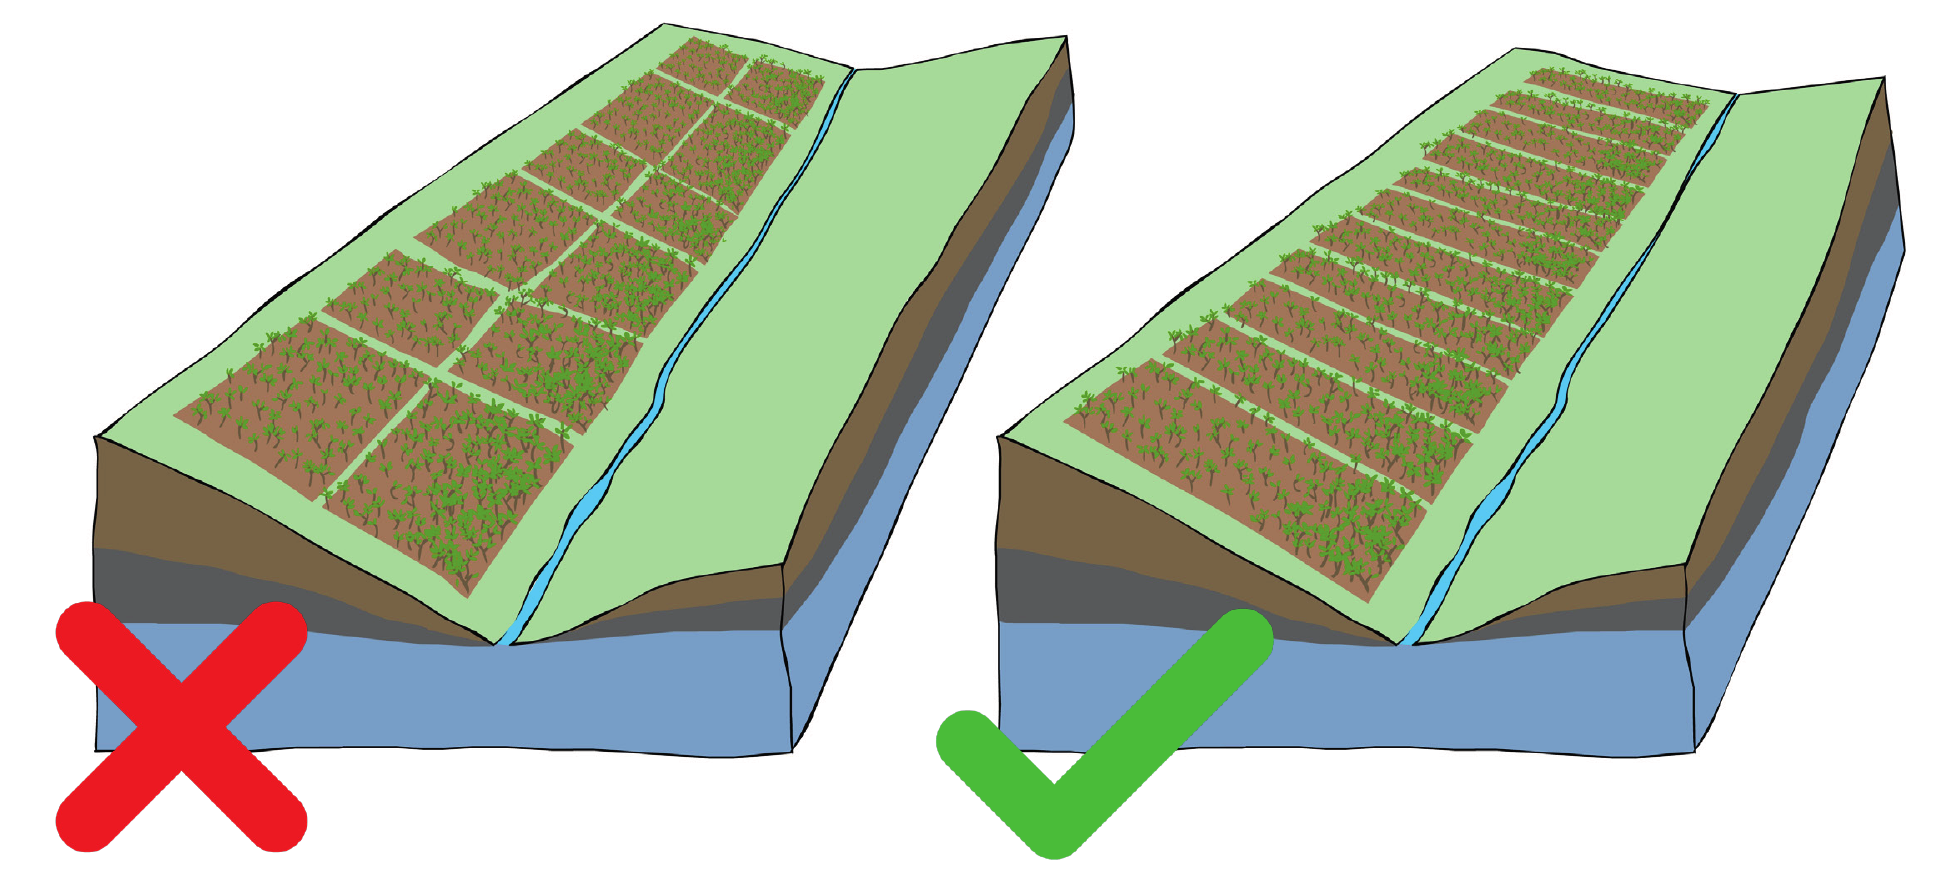
\includegraphics[width=0.95\linewidth]{./images/blocking_concept} \end{center}
\end{frame}

\begin{frame}{Randomization}
\protect\hypertarget{randomization}{}
\begin{itemize}[<+->]
\tightlist
\item
  The purpose of randomization is to prevent \emph{systematic and
  personal biases} from being introduced into the experiment by the
  experimenter.
\end{itemize}

\begin{itemize}[<+->]
\tightlist
\item
  Lack of a random assignment of experimental material or subjects
  leaves the experimental procedure open to \alert{experimenter bias}.

  \begin{itemize}[<+->]
  \tightlist
  \item
    a horticulturist may assign his or her favorite variety of
    experimental crop to the parts of the field that look the most
    fertile,
  \item
    a medical practitioner may assign his or her preferred drug to the
    patients most likely to respond well.
  \end{itemize}
\item
  The preferred variety or drug may then appear to give better results
  no matter how good or bad it actually is.
\end{itemize}
\end{frame}

\begin{frame}{}
\protect\hypertarget{section-4}{}
\begin{itemize}[<+->]
\tightlist
\item
  Consider an experiment to compare the effects on blood pressure of
  three exercise programs, where each program is observed four times,
  giving a total of 12 observations. Now, given 12 subjects, imagine
  making a list of all possible assignments of the 12 subjects to the
  three exercise programs so that 4 subjects are assigned to each
  program. (There are \(\frac{12!}{(4!4!4!)}\), or 34,650 ways to do
  this.) If the assignment of subjects to programs is done in such a way
  that every possible assignment has the same chance of occurring, then
  the assignment is said to be a completely random assignment.
\item
  A random assignment in experimental design is achieved through a
  random number generator or a random number table.
\end{itemize}

\begin{itemize}[<+->]
\tightlist
\item
  The most common random number generators on computers or calculators
  generate n-digit real numbers between zero and one. Single digit
  random numbers can be obtained from an n-digit real number by reading
  the first digit after the decimal point. Pairs of digits can be
  obtained by reading the first two digits after the decimal point, and
  so on.
\end{itemize}
\end{frame}

\begin{frame}{Randomization: An Exercise in Spreadsheet}
\protect\hypertarget{randomization-an-exercise-in-spreadsheet}{}
\begin{center}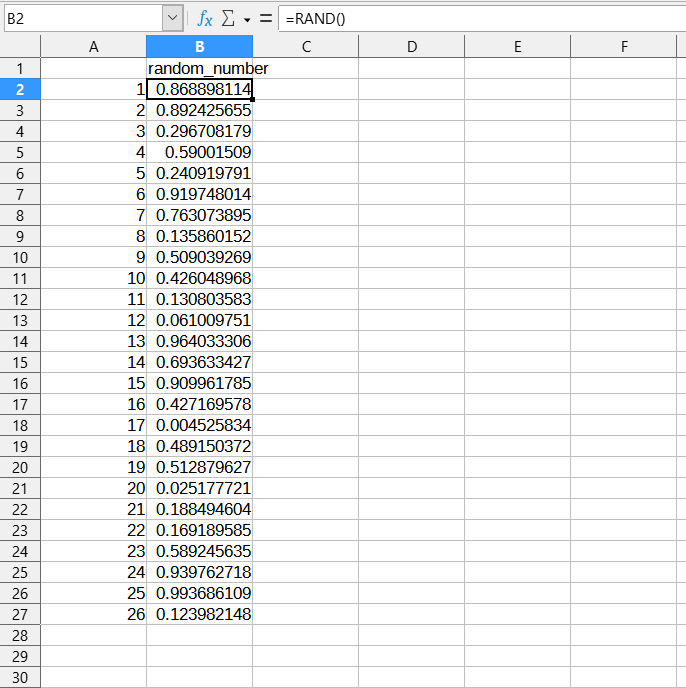
\includegraphics[width=0.45\linewidth]{./images/random_number_generation_spreadsheet} \end{center}
\end{frame}

\begin{frame}{Comparison and local control}
\protect\hypertarget{comparison-and-local-control}{}
\begin{itemize}[<+->]
\tightlist
\item
  Experiments are controlled so as to isolate the differences between
  the treatments of interest, and to minimize extraneous variability so
  as to enable the sharpest possible statistical analyses (e.g., narrow
  confidence intervals or powerful tests).
\item
  In many instances, this high degree of control means that the data
  collected are actually representative of only a very special
  situation, reflecting the particular laboratory procedures, batch of
  experimental material, et cetera, used in the performance of the
  experiment. As a result, meaningful inferences usually need to be
  based on comparisons within an experiment, with the idea that anything
  unusual, but common, to all trials in the experiment will ``cancel
  out'' in the analysis.
\end{itemize}
\end{frame}

\begin{frame}{}
\protect\hypertarget{section-5}{}
\begin{columns}[T, onlytextwidth]
\column{0.6\textwidth}
\begin{itemize}
\item "Comparison" often leads to the inclusion of one or more experimental controls.
  \begin{itemize}
  \footnotesize
  \item For example, in addition to the four carefully defined "experimental treatments", while evaluating pipeline varieties, one or two "locally adapted" cultivars are included so as to provide a comparison to what might have happened in a "normal" scenario or how would the "local check" perform in controlled experimental conditions.
  \end{itemize}
\item A large difference between responses form these treatment and "checks" could indicate unanticipated influences of the experimental procedure \textit{per se}; a small or negligible difference might be viewed as support for the investigators' intent that "checks" are a reasonable representation for genotypes suited to the target environment.
\end{itemize}
\column{0.4\textwidth}


\begin{center}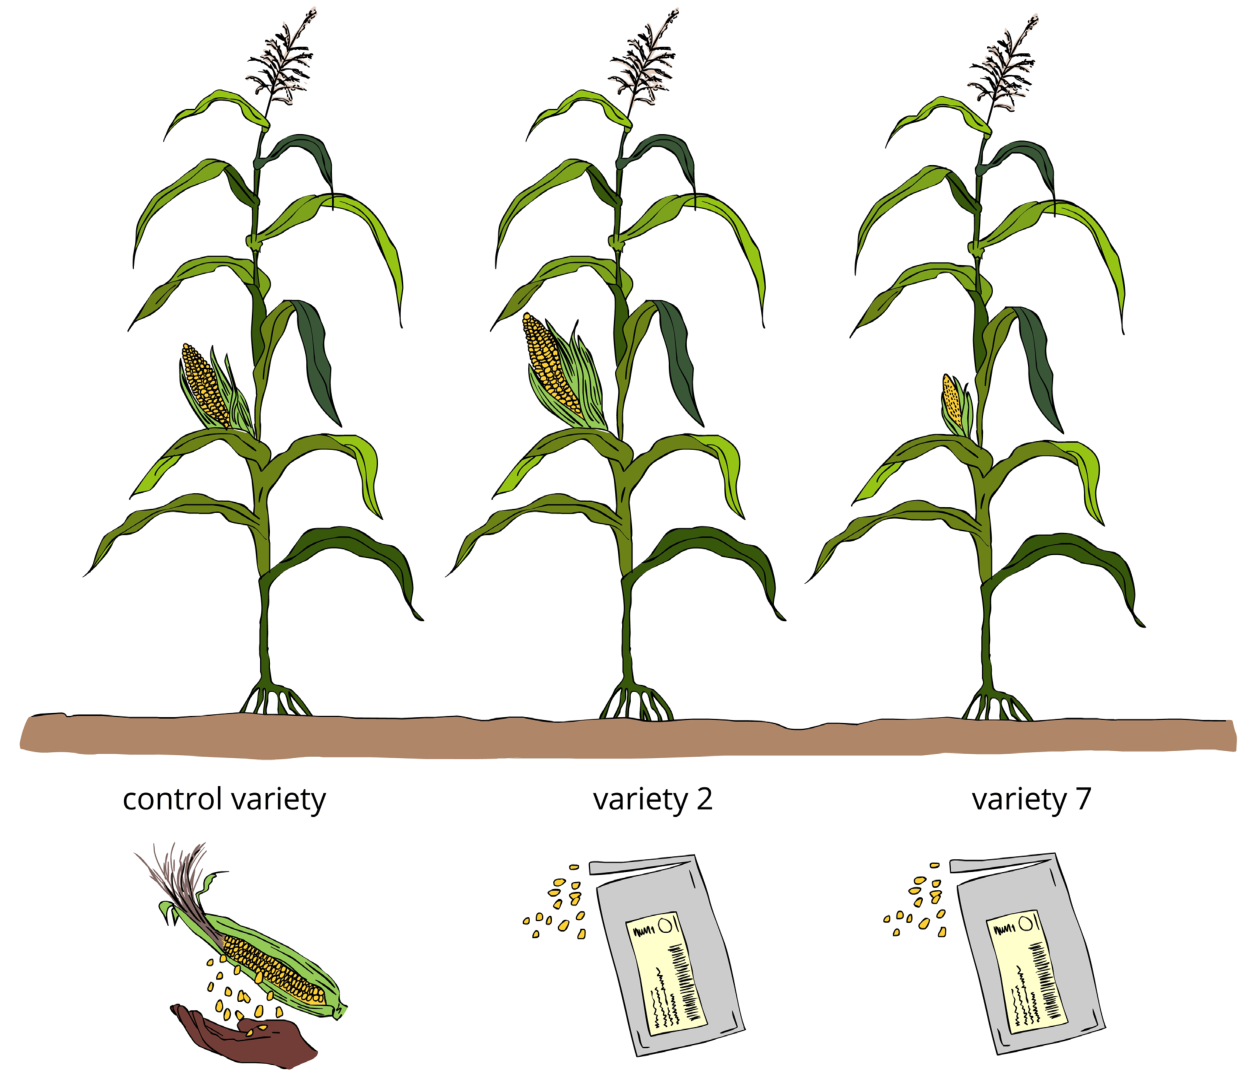
\includegraphics[width=0.98\linewidth]{./images/local_check} \end{center}

\end{columns}
\end{frame}

\hypertarget{interpretation-of-results}{%
\section{Interpretation of results}\label{interpretation-of-results}}

\begin{frame}{Interpretation of results}
\protect\hypertarget{interpretation-of-results-1}{}
\begin{itemize}[<+->]
\tightlist
\item
  Design of experiments enable uniformly control (or adjustment) of
  environmental factors that are not a part of the treatments being
  evaluated.
\item
  This uniformity is both an advantage and a weakness of a controlled
  experiment.
\item
  Clearly the result of an experiment is, applicable only to conditions
  that are the same as, or similar to, that under which the experiment
  was conducted.
\end{itemize}
\end{frame}

\begin{frame}{}
\protect\hypertarget{section-6}{}
\begin{columns}
\column{0.8\textwidth}
A glass could be:
\begin{itemize}
\footnotesize
\item Half full (optimist)
\item Half empty (pessimist)
\item Twice as big as it needs to be (project manager)
\item Half the required amount of liquid for it to overflow (realist)
\end{itemize}
Idiosyncrasies:
\begin{itemize}
\footnotesize
\item How it can be half full or half empty ? FULL is \alert{FULL} and EMPTY is \alert{EMPTY}.
\item If completely full, \alert{half with air and half with water}.
\item Only optimistic can \alert{see half empty}, how can they be a pessimist ?
\item Half full could be the answer, if you think you have \alert{enough} there.
\item Half empty could be the answer, if what you have is \alert{not sufficient}.
\end{itemize}
\column{0.2\textwidth}


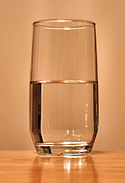
\includegraphics[width=0.8\linewidth]{./images/half-empty-glass} 

\end{columns}
\end{frame}

\hypertarget{bibliography}{%
\section{Bibliography}\label{bibliography}}

\begin{frame}{References}
\protect\hypertarget{references}{}
\end{frame}

\end{document}
